

\chapter{Impurity resistance of dense metal membranes under hydrogen impurities}
\section {Abstract}
In this chapter a number of dense palladium alloy membranes were synthesised on a YSZ substrate using a combination of electroless plating and magnetron sputtering in order to determine which membrane compositions resisted impurities. 

The permeability of the synthesised membranes, in addition to a commercial membrane were tested under a variety of ISO 14687-2 impurities in order to determine which alloy composition was most suitable for use as a membrane material for hydrogen impurity enrichment, where low reactivity with impurities present in hydrogen samples are required. Of the tested membranes the best performing compositions were PdAuAg, PdAuCu and PdCuZr which only showed a 27\%, 25\% and 26\% drop in permeability under atmospheres containing 10 ppm of non-sulphurous, and 2 ppm of sulphurous impurities typically expected to be found in hydrogen derived from steam methane reforming.  This indicates that these alloys are most suitable for metrology purposes due to their low reactivity. 

\section{Introduction}
In order to improve the accuracy and the cost of hydrogen impurity enrichment a suitable membrane composition must be found. In addition to this all previous studies used a commercial palladium-based membrane and in all cases it was noted that certain impurities reacted with the membrane. This interaction had the result of changing the composition of the enriched gas muxture and therefore reducing the final accuracy of the measurement. \cite{Murugan2014, Ahmed2010} The self-supported commercial membranes used in both studies are also generally between 20-100 $\mu$m in order to provide sufficient mechanical strength for a membrane. However, for palladium membranes to be economical this thickness must be reduced to about 1-5 $\mu$m giving the added benefit of greater flux and therefore lower enrichment times. 

Palladium alloy membranes are generally created by forming an alloy with silver, copper or gold. By doing this the hydrogen embrittlement effect can be effectively mitigated. Using alloys has the added benefits of decreasing the overall amount of palladium required in the film, driving up their cost effectiveness, and in some cases increasing the flux of the membrane to higher levels achievable than a pure palladium membrane. In the previous chapter a number of membrane compositions were identified to be able to resist certain classes of ISO 14687-2 impurities. The best membranes being identified as PdAu\textsubscript{20} and PdAu\textsubscript{20}Cu\textsubscript{10} for carbonaceous impurities. For sulphur containing impurities PdCu\textsubscript{20}Zr\textsubscript{10}, PdAu\textsubscript{20}Zr\textsubscript{10}, and PdAu\textsubscript{20}Cu\textsubscript{10} were the most resistent to binding with H\textsubscript{2}S.In this chapter these membranes will be manufactured and tested under environments containing these gases in order to verify these results, and quantify the level of reactivity. In addition to these alloys, PdCu\textsubscript{20}Ag\textsubscript{10} and PdAu\textsubscript{20}Ag\textsubscript{10} will be synthesised due to their strong performance in the previous chapter. PdAg\textsubscript{23}, PdCu\textsubscript{20} and PdCu\textsubscript{40} will also be synthesised as these are popular membrane compositions in literature and act as a good benchmark in addition to the commercial membrane. Unfortunately the PdAuZr composition could not be manufactured due to the high cost associated with sputtering gold.

Palladium alloy membranes will be deposited onto porous YSZ supports using both electroless plating  and closed field unbalanced magnetron sputter ion plating as described in sections \ref{exp-elpproc} and \ref{exp-msproc}. This will have the combined effect of reducing the amount of palladium used, driving down their cost, and  increasing the flux, and therefore reducing the time taken to enrich a hydrogen sample. The degree of interaction of impurities with the surface of the membrane will be quantified using a three-step experimental procedure. The pure hydrogen flux of each membrane composition will be measured and the membranes hydrogen permeability calculated as a base line. The following two permeation tests will measure the change in permeability resulting from introducing part-per-million level impurities into the gas sample. The change in permeability which results from this will act as a measure for the membranes tendency to interact with different impurity types. Additionally, at all three testing stages, X-ray photoelectron spectroscopy (XPS) will be performed on the surface of the membranes to investigate how the composition on the surface of the membrane changes when exposed to each impurity environment. This will allow the alloy segregation behaviour to be observed, and more importantly, quantify the amount of sulphur which has reacted with the surface of the membrane. 

\section{Results and Discussion}
\subsection{Membrane characterisation}

Figure \ref{fig:1} (a)-(g) shows the cross-sectional SEM images of the manufactured membranes.  The thickness of the fabricated membranes are shown in \ref{results:1} and ranged from 573 nm to 1.579 $\mu$m. In general thinner layers were achieved using electroless plating although theoretically sub-micron layers are possible through magnetron sputtering, examples of this being SINTEF’s patented sputtering process.\cite{Peters2011} The integrity of the manufactured membranes was measured using the procedure laid out in section \ref{exp-MatTest}. All membranes showed no leakage when pressurised to 10 bar indicating that all membranes were uniform, pinhole free and therefore suitable for hydrogen separation. \cite{GouveiaGil2015}

\begin{figure}
    \centering
    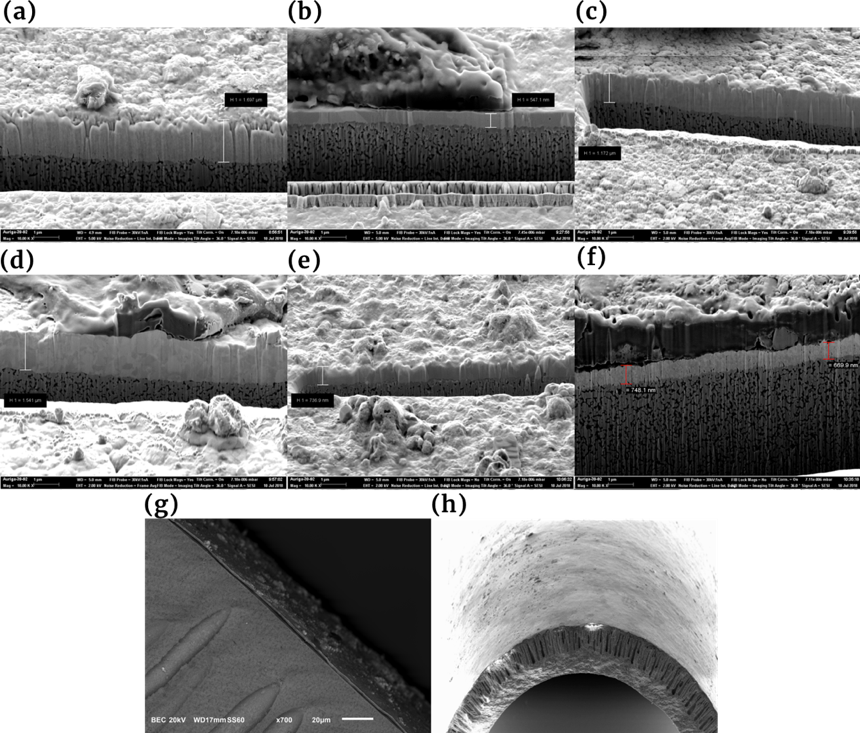
\includegraphics[width=\linewidth, height=0.9\textheight,keepaspectratio]{figures/Semxsect.png}
    \caption{SEM images of fabricated membranes (a) PdCu (fcc) (Sputtering) (b) PdAg (ELP) (c)PdAu (ELP) (d) PdCuZr (Sputtering) (e) PdAgAu (ELP) (f) PdCuAg (ELP) (g) PdCu (bcc) (Sputtering) (h) typical cross section}
    \label{fig:1}
\end{figure}

The surface composition of each membrane was measured by XPS and is shown in Table \ref{results:1}. A wide range of compositions were fabricated. From phase data on the PdCu system \cite{Roa2003, Nayebossadri2013} both varieties of PdCu membranes (bcc phase and fcc phase) were successfully fabricated. 

\begin{table}[]
    \centering
    \caption{Membrane compositions analysed by EDS and their thickness measured using FIB-SEM}
    \label{results:1}
    \resizebox{\textwidth}{!}{\begin{tabular}{@{}cccccccc@{}}
    \toprule
    \multicolumn{1}{c}{\multirow{2}{*}{Membrane ID}} & \multirow{2}{*}{Manufacturing technique} & \multicolumn{5}{c}{Composition (wt\%) (+- 1\% Relative)} & \multirow{2}{*}{Thickness (um)} \\
    \multicolumn{1}{c}{}                             &                                          & Pd        & Cu        & Ag        & Au        & Zr       &                                 \\ \midrule
    PdCu (Fcc)                                        & Magnetron Sputtering                     & 76.24     & 23.76     & -         & -         & -        & 1.679                           \\
    PdCu (Bcc)                                        & Magnetron Sputtering                     & 43.24     & 56.64     & -         & -         & -        & 1.664                           \\
    PdCuZr                                            & Magnetron Sputtering                     & 72.10     & 14.46     & -         & -         & 13.54    & 1.541                           \\
    PdAg                                              & Electroless Plating                      & 65.55     & -         & 34.45     & -         & -        & 0.573                           \\
    PdAu                                              & Electroless Plating                      & 74.7      & -         & -         & 25.3      & -        & 1.172                           \\
    PdCuAg                                            & Electroless Plating                      & 72.1      & -         & 8.27      & 19.58     & -        & 0.867                           \\
    PdCuAu                                            & Electroless Plating                      & 63.90     & 13.6      & -         & 22.1      & -        & 1.545                           \\
    PdAuAg                                            & Electroless Plating                      & 60        & -         & 11.2      & 28.3      & -        & 0.736                           \\ \bottomrule
    \end{tabular}}
\end{table}

% Silver is the most popular dopant for palladium membranes and forms a stable alloy with palladium at concentrations greater than 20 wt\%, with the optimal composition occurring at 23 wt\%. On top of mitigating the effects of hydrogen embrittlement, a $~$60\% increase in permeability is observed when compared to pure Pd membranes. Despite having enhanced permeation properties, PdAg is still susceptible to poisoning, in particular from sulphurous compounds which can form both Pd\textsubscript{4}S and Ag\textsubscript{5}Pd\textsubscript{10}S\textsubscript{5}. A composition of Pd\textsubscript{64.9}Ag\textsubscript{35.1} wt\% was achieved, which, while higher than the desired composition of Pd\textsubscript{77}Ag\textsubscript{23} wt\%, was determined adequate for the purposes of this study.

% Copper is another widely studied binary alloy which is known to suppress hydrogen embrittlement. Alloying with copper also has the advantage that it reduces the cost of the membrane by a larger amount than most other metals and through improving the membranes sulphur resistance. The maximum permeability of a palladium copper membrane occurs at the composition Pd\textsubscript{60}Cu\textsubscript{40} wt\% and this is due to the formation of a bcc lattice rather than the fcc lattice commonly seen in pure palladium and most binary alloys. \cite{She2014} Temperature cycling has previously been performed on this alloy composition and it has been found that the bcc crystalline configuration has a higher permeability than the fcc phase. \cite{Dolan2010} This behaviour is due to the increased number of hcp adsorption sites which hydrogen has a slight preference for, and the bcc structure allowing faster diffusion through the bulk of the membrane. \cite{Wilcox2010} Conversely the fcc structure has a higher impurity resistance than the bcc structure, particularly for H\textsubscript{2}S. \cite{She2014, D.T.Hughes1978} Pd\textsubscript{44}Cu\textsubscript{66} and Pd\textsubscript{65.5}Cu\textsubscript{34.5} wt \%  membranes were manufactured using magnetron sputtering which were in the range for bcc and fcc phases respectively.

% PdAu alloys see a slight increase in permeability, up to 30\% more than pure Pd \cite{Atsonios2015}, with gold additions up to 20\%, after which the permeability rapidly decreases. While alloying with gold does not improve the permeability much compared to silver or copper, gold alloys show greatly improved sulphur resistance. \cite{Chen2010} The synthesised membrane was found to have the composition  Pd\textsubscript{74.7}Au\textsubscript{25.3} which, while containing a high amount of gold resulting in lower permeation, will have a higher impurity resistance. 

\subsection{Hydrogen permeation}
Table \ref{results:2} shows the hydrogen permeation through the 9 tested membranes at steady state after 12 hours of operation. As expected, hydrogen permeation flux increases with the elevated temperatures. Moreover, the mass transfer resistance of the substrate will not represent major limitations since its gas transport resistance is negligible compared to that of the dense palladium alloy layer \cite{GouveiaGil2015}. Deposited layers were all on the scale of 0.5-2 $\mu$m which from previous research indicates the main rate limiting step in hydrogen permeation being the thickness of the membrane layer. \cite{NathanW.Ockwig2007a} The palladium copper alloy which was in the bcc phase showed the highest hydrogen permeability of all the synthesised membranes which was expected as discussed in section \ref{lit-pdreview}. The membrane which showed the lowest hydrogen permeability was the PdCuZr membrane, this is likely due to the combined effects of the alloy having the lowest concentration of palladium compared to the other synthesised membrane, increasing the transport resistance of the membrane, and this composition having a lower preference to hydrogen binding as all other palladium alloys as predicted in the simulations performed in section \ref{dft-Hsection} and shown in figure \ref{dft-h2ads}. The PdAu and PdAuAg membranes both showed low permeabilities. Gold as an alloying material traditionally does not show much increase in permeability \cite{Chen2010}  but is instead used to suppress the effects of impurities on the membrane, \cite{Chen2010} which is the main goal of this study. Despite the fact that the commercial membrane is also based on PdAgAu, the membrane manufactured through electroless plating has a lower permeability due to the high gold concentration. It is likely that the concentration of silver in the commercial membrane is closer to 23\%, which is the optimal value for hydrogen permeation, and it’s gold concentration is much lower than the electroless plated membrane. Both PdCuAg and PdCuAu had reasonably high hydrogen permeabilities. While none of these membranes showed a hydrogen permeability as high as the commercial alloy, it should be noted that the commercial membrane had a much larger thickness resulting in a much higher cost and lower flux values than the composite membranes. 

\begin{table}[]
    \centering
    \caption{Pure hydrogen permeability of studied alloy membranes under pure hydrogen at 300\textdegree C and 1 bar pressure differential}
    \label{results:2}
    \begin{tabular}{@{}cc@{}}
        \toprule
        \multicolumn{1}{c}{Membrane ID} & \begin{tabular}[c]{@{}c@{}}Permeability\\ ($mol\:m^{-1} s^{-1} pa^{1/2} \times 10^{-8}$)\end{tabular} \\ \midrule
        PdCu (Fcc)                       & 1.30                                                                                               \\
        PdCu (Bcc)                       & 1.68                                                                                               \\
        PdCuZr                           & 0.14                                                                                               \\
        PdAg                             & 0.94                                                                                               \\
        PdAu                             & 0.33                                                                                               \\
        PdCuAg                           & 1.22                                                                                               \\
        PdCuAu                           & 1.43                                                                                               \\
        PdAuAg                           & 0.19                                                                                               \\
        Commercial (REB)                 & 5.71                                                                                               \\ \bottomrule
        \end{tabular}
\end{table}


\subsection{Impurity reactivity}

\begin{table}[]
\centering
\caption{Permeability results for all membranes under both impurity conditions}
\label{results:3}
\begin{tabular}{@{}cccccl@{}}
\toprule
\multirow{2}{*}{Membrane ID} & \multicolumn{3}{c}{\begin{tabular}[c]{@{}c@{}}Permeability\\ ($mol\:m^{-1} s^{-1} pa^{1/2} \times 10^{-8}$)\end{tabular}} & \multicolumn{2}{c}{\% Drop} \\
                             & Pure H\textsubscript{2}  & Non-Sulphur & Sulphur & Non-sulphur    & Sulphur    \\ \midrule
PdCu (Fcc)                   & 1.30     & 0.22        & 0.185   & 80\%           & 86\%       \\
PdCu (Bcc)                   & 1.68     & 0.721       & 2.47    & 55\%           & 85\%       \\
PdCuZr                       & 0.14     & 0.12        & 0.101   & 12\%           & 26\%       \\
PdAg                         & 0.94     & 0.117       & 0.007   & 88\%           & 92\%       \\
PdAu                         & 0.33     & 0.165       & 0.215   & 51\%           & 35\%       \\
PdCuAg                       & 1.22     & 0.48        & 0.299   & 61\%           & 75\%       \\
PdCuAu                       & 1.43     & 0.789       & 1.07    & 45\%           & 25\%       \\
PdAuAg                       & 0.19     & 0.163       & 0.142   & 16\%           & 27\%       \\ \bottomrule
\end{tabular}
\end{table}

Table \ref{results:3} shows the results of hydrogen permeation under the presence of the two different impurity conditions discussed in Table \ref{results:3} compared to the pure hydrogen permeability values shown in Table \ref{results:2}. The permeability data was taken once the flux had reached steady state after 12 hours of operation. For all membranes there was a reduction in permeability when the membranes were exposed to impurities. The magnitude of this reduction compared to the pure hydrogen permeability is used as an indication of the degree of interaction between the membrane and the impurities.  Table \ref{results:4} shows the composition of each membrane in between each test in order to measure permanent surface reactions and segregation behaviour of the alloys under the chosen impurities. 

\subsubsection{Binary alloys}
In non-sulphur tests the PdAg binary alloy was the worst performing, with the permeability dropping by 88\% of its original value. This was expected as the addition of silver to a palladium system, while effective at increasing the permeability, does not contribute much to impurity resistance. \cite{Peters2016b} This was further supported by the results of the sulphur tests where the permeability dropped by 92\% and composition analysis in Table \ref{results:4} showing that sulphur was present in 42\% of the surface. The PdAg alloy also showed a large degree of segregation behaviour under non-sulphur impurities which likely contributed to the large reduction in flux, with silver concentration increasing to 75\% at the top 10 nm of the sample, resulting in a large drop in permeability. 

Interestingly the PdCu membrane with a composition in the bcc phase showed higher resistance to non-sulphurous impurities than the fcc phase, with the former only experiencing a 55\% drop in permeability compared to an 80\% drop in permeability in the latter. This again seems to be a result of the segregation behaviour of the alloy, with the PdCu alloy in the fcc phase experiencing a large amount of segregation, with the palladium concentration increasing to around 90\% on the retentate side. Conversely the PdCu composition in the BCC phase membrane only changed slightly. The XPS analysis showed that while the reactivity of sulphur on the surface of both copper based binary membranes was of a similar magnitude, the BCC phase had a slightly lower resistance, with 29\% of the surface containing sulphur after exposure to sulphurous impurities as opposed to the 25\% shown by the fcc phase alloy.

The PdAu alloy showed the best impurity resistance out of the binary alloys tested under both impurity conditions, with only a 51\% and 35\% drop in permeability under non-sulphur and sulphur conditions respectively and only a 12\% concentration of sulphur was observed on the surface after XPS analysis. The alloy showed slight segregation of gold away from the permeate surface under non-sulphur impurity conditions likely due to the fact the difference in interaction strength between gold and palladium with the components of the gas mixture varies widely, with many gases preferentially adsorbing on palladium \cite{Gade2011}.

\begin{landscape}
\begin{table}[]
    \centering
    \caption{XPS composition analysis of the palladium alloy membrane surfaces after impurity tests}
    \label{results:4}
    \begin{tabular}{@{}ccccccccccccccccc@{}}
    \toprule
    \multirow{2}{*}{Membrane ID} & \multicolumn{5}{c}{Pure Hydrogen Exposure} & \multicolumn{5}{c}{Non-Sulphur Exposure} & \multicolumn{6}{c}{Sulphur Exposure} \\
                                 & Pd     & Ag     & Au     & Cu     & Zr     & Pd      & Ag     & Au    & Cu     & Zr   & Pd    & Ag  & Au  & Cu   & Zr & S    \\ \midrule
    PdCu (Fcc)                   & 65.5   & -      & -      & 35.5   & -      & 92.5    & -      & -     & 7.5    & -    & 67.5  & -   & -   & 7.5  & -  & 25   \\
    PdCu (Bcc)                   & 44     & -      & -      & 66     & -      & 54.85   & -      & -     & 45.15  & -    & 40    & -   & -   & 31   & -  & 29   \\
    PdCuZr                       & 63.6   & -      & -      & 22.6   & 13.8   & 64.4    & -      & -     & 27.5   & 8.5  & 54.2  & -   & -   & 27   & 8  & 10.8 \\
    PdAg                         & 65.5   & 34.5   & -      & -      & -      & 25      & 75     & -     & -      & -    & 29    & 29  & -   & -    & -  & 42   \\
    PdAu                         & 75     & -      & 25     & -      & -      & 82.9    & -      & 17.1  & -      & -    & 71    & -   & 16  & -    & -  & 13   \\
    PdCuAg                       & 64.6   & 9.1    & -      & 26.3   & -      & 8.6     & 8.9    & -     & 82.5   & -    & 6     & 5   & -   & 64   & -  & 25   \\
    PdCuAu                       & 63.9   & -      & 22.5   & 13.6   & -      & 84.9    & -      & 1.46  & 13.6   & -    & 65.3  & -   & 1   & 18.5 & -  & 15.2 \\
    PdAuAg                       & 60     & 11.7   & 28.3   & -      & -      & 47.2    & 49.8   & 3     & -      & -    & 52    & 35  & 1   & -    & -  & 12   \\ \bottomrule
    \end{tabular}
    \end{table}
\end{landscape}
\subsubsection{Ternary alloys}
Five ternary alloy compositions were tested including the commercial alloy. The commercial alloy had the highest permeability of all ternary alloys with a value of 5.71 mol m\textsuperscript{-1} s\textsuperscript{-1} pa\textsuperscript{-0.5}x10\textsuperscript{-8} under pure hydrogen and 4.28 mol m\textsuperscript{-1} s\textsuperscript{-1} pa\textsuperscript{-0.}5x 10\textsuperscript{-8}  under non-sulphur conditions, a drop in permeability of 25\%. However, the commercial membrane nearly lost all of its permeability under sulphurous conditions. The PdAuAg membrane manufactured through electroless plating performed better under both impurity conditions than the commercial alloy despite being based on the same composition, only seeing a 16\% and 27\% drop in hydrogen permeability under non-sulphur and sulphur conditions respectively compared to a 25\% and 96\% drop shown by the commercial alloy. The high levels of gold likely contributed to the low levels of sulphur on the surface of the electroless plated PdAuAg membrane. These results indicate that the composition of the commercial membrane, while ideal for separation, does not contain enough gold to withstand the levels of sulphur impurities expected for analytical purposes. 

The worst performing ternary alloy was the PdCuAg alloy which showed large permeability drops under all conditions, 61\% under non-sulphur and 75\% under sulphurous conditions. In addition to these, large degrees of segregation were observed under non-sulphur impurities, with the palladium concentration at the surface dropping to 8.5 wt\%, showing that the alloy is not completely stable under the varying conditions expected during analytical purposes.  

Both gold containing ternary alloys, PdAuAg and PdCuAu, performed well under sulphur conditions, with the PdCuAu alloy only reducing in permeability by 25\% and the PdAgAu membrane by 27\%. The PdCuAu membrane however had a stronger interaction with non-sulphur impurities, indicated by the permeability drop of 45\% when exposed to the non-sulphur containing gas sample. This drop is likely due to the segregation of palladium to the surface with the XPS data indicating an increase of palladium to the surface to 84.9 wt\% from 63.9\%. The best performing ternary membrane was the PdCuZr membrane which showed the smallest drop in permeability of only 12\% non-sulphur conditions, and a permeability percentage drop of 26\% under sulphur conditions which on a similar magnitude to that of the gold containing alloys.
\begin{landscape}
    
\begin{figure}
    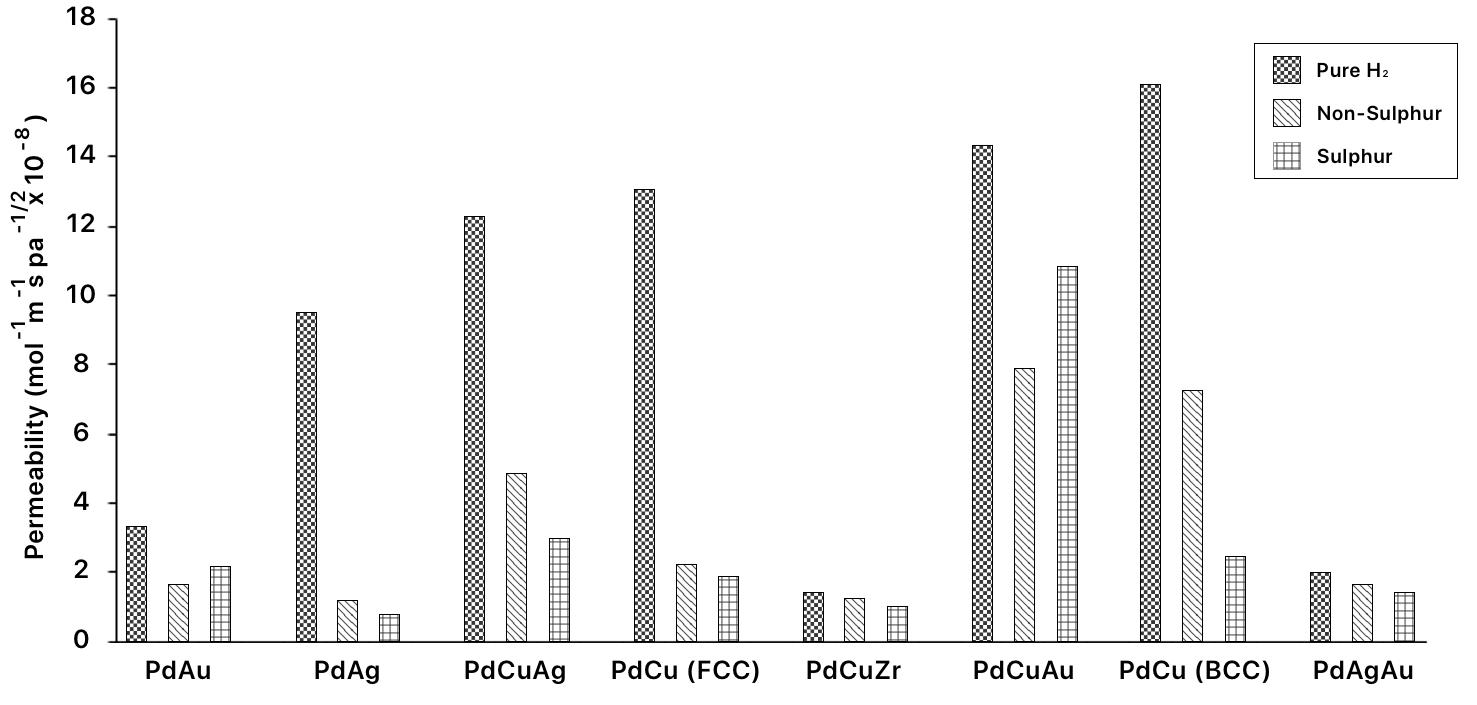
\includegraphics[width=\linewidth]{figures/permeabilitychart.png}
    \caption{Permeability data for pure hydrogen, non-sulphur, and sulphur permeation tests}
    \label{permgraph}
  \end{figure}
\end{landscape}

\subsubsection{Segregation behaviour}
All membranes tested showed some degree of segregation with the two thinnest membrane samples, PdAg (0.573 micron), PdAuAg (0.736  micron) and PdCuAg (0.873 micron) all showing the highest degrees of segregation. While this may still be a property of the alloy compositions it may also indicate that sub-micron palladium alloys layers are unstable and there may be a minimum thickness for alloys, below which the membrane layer is unstable and frequently varies during operation.

\subsection{Relationship to DFT results}
The previous chapter attempted to use DFT generated binding energies to predict the perfomance of alloy composistions in environments containing ISO 14687-2 impurities. While a useful analysis it appears in some cases that these results were not completely correct and could be improved in further studies. 

For carbonaceous environments the model predicted that PdAu20 and PdAuCu would be the best performing alloys. PdAuCu experienced a 45\% drop in permeability under carbonaceous environments while PdAu\textsubscript{20} experienced a 51\% drop. Which while showing reasonable resistance, were inferiour to both the PdCuZr and PdAuAg alloys which only experienced a 12\% and 16\% drop respectivley. For the PdAuAg alloy the model did indeed predict that it would resist adsorption to these impurities, and agrees with the conclusion of this alaysis that the addition of gold and silver improves the alloys resistence to carbonaceous impurities. However appears to be completely incorrect, with all models predicting that the alloy would be more susceptible to poisoning. 

The model fared better when predicting the influence of sulphurous impurities on the surface of the membrane. The model successfully predicted that both PdCuAu and PdCuZr alloys would be the most resistent to sulphurous environments. The model appears to be accurate in predicting how the other alloys would react in the environment, indicating the PdAg, PdCuAg, and both FCC and BCC PdCu alloys would perform poorly and see severe levels of sulphur poisoning. It should be noted that many of the results in this section were close and other alloys which performed reasonably well against sulphur poisoning (PdAu\textsubscript{20} and PdAuAg) could be as a result of the error between simulations. 

The DFT simulations were a useful tool in predicting the sulphur resistance of the alloys, however when used to predict the behaviour of weaker adsorbing compounds, such as the carbonaceous impurities, it appears to break down. This is likely due to the fact that DFT is not as effective at simulating the behaviour of weaker bonds as discussed in section \ref{lit-DFTLIMS}. Alternative methods should be explored if these interactions are to be predicted.

\section{Conclusion}
In order to identify a suitable palladium alloy composition for hydrogen impurity enrichment, eight different membrane compositions were manufactured and tested under three different hydrogen conditions against a commercial palladium membrane. Two different measures were used to compare the membrane compositions suitability for hydrogen impurity enrichment, the permeability deviation from the pure hydrogen permeability was used as an initial indicator of interaction between the alloy and impurities, and the surface composition was measured to detect any impurities which had permanently reacted with the membrane. 

The best performing membrane, and therefore the most suitable for hydrogen impurity enrichment was the PdCuZr alloy, which only showed a 12\% and 26\% drop in permeability under non-sulphur, and sulphur conditions, and low levels of sulphur on the surface. The permeability of this alloy was low, however, surface areas could easily be scaled up to increase the speed of hydrogen enrichment. 

In the following chapter this membrane will be used in the design of the hydrogen impurity enrichment device and it's performance measured when tested with a real hydrogen fuel sample.

\bibliographystyle{unsrtnat}
\bibliography{library.bib}